\section{Governing equations and numerical models}\label{model} 
The system of interest is a self-gravitating, inviscid fluid disc
orbting a central star of mass $M_*$. We will mainly consider two-dimensional
(2D, or razor-thin) discs in favour of numerical
resolution, but have also carried out some three-dimensional (3D) disc
simulations. Hence, for generality we describe the system in
3D. We use both cylindrical $(R,\phi,z)$ and spherical polar
coordinates $(r,\theta,\phi)$ centred on the star. 
The governing fluid equations in 3D are  
\begin{align}
  &\frac{\p\rho}{\p t} + \nabla\cdot\left(\rho\bm{v}\right) =
  0,\label{cont_eq}\\
  &\frac{\p\bm{v}}{\p t} + \bm{v}\cdot\nabla\bv = -\frac{1}{\rho}\nabla
  p -\nabla \Phi_\mathrm{tot}\label{mom_eq},\\ 
  & \nabla^2\Phi_d = 4 \pi G \rho \label{poisson}, 
\end{align}
where $\rho$ is the mass density, $\bm{v}=(v_r,v_\theta,v_\phi)$ the
fluid velocity, $p$ is the pressure and the total potential
$\Phi_\mathrm{tot} = \Phi_* + \Phi_d$ consists of that from the
central star, 
\begin{align}
  \Phi_*(r) = -\frac{GM_*}{r}, 
\end{align}
where $G$ is the gravitational constant,  and the disc potential
$\Phi_d$. We further assume a locally 
isothermal equation of state 
\begin{align}
  p = c_s^2(R)\rho,
\end{align}
where the sound-speed is given by $c_s=H\Omega_k$, where $H=hR$ is the
disc scale-height with constant aspect-ratio $h$ chosen below, and
$\Omega_k=\sqrt{GM_*/R^3}$ is the midplane Keplerian frequency.  

We have purposefully adopted the simplest model that was found to
develop one-arm spirals in discs with radial structure. The indirect
potential associated with the non-inertial reference frame is
neglected to avoid complications arising from the motion of the
central star. For the adopted disc masses $M_d\lesssim 0.1 M_*$, this
effect is not expected to be significant. The locally isothermal
equation of state allows us to apply standard linear density wave
theory for results interpretation. 
%This allows us to consider
%an isolated disc.   

The 2D disc equations are obtained by replacing $\rho$ with the surface
mass density $\Sigma$ and $p$ with the vertically-integrated pressure
$\Pi$ in the continuity and momenta equations, and the 2D fluid
velocity $\bm{v}=(v_R,v_\phi)$ is evaluated at the midplane, as are
the forces from the potential. In the Poisson equation, $\rho$ is
replaced by $\Sigma\delta(z)$, where $\delta(z)$ is the
delta function. 

\subsection{Disc model and initial conditions}
%We consider a smooth disc which contains a surface density bump
%between $R\in[R_{d1},R_{d2}]$, mimicking mass built-up in a dead
%zone. 
We adopt a modified power-law disc with surface
density profile 
\begin{align}
  \Sigma(R) = \Sigma_\mathrm{ref} \left(\frac{R}{R_0}\right)^{-s}\times B(R;
  R_{d1}, R_{d2}, \epsilon, \delta R_d), 
\end{align}
where $R_0$ is a reference cylindrical radius and $s$ is the power-law
index describing the smooth disc, and $\Sigma_\mathrm{ref}$ is a
surface density scale chosen by specifying $Q_\mathrm{out}$,
the Keplerian Toomre parameter at $R=R_{d2}$,
\begin{align}
  Q_\mathrm{out} = \left.\frac{c_s\Omega_k}{\pi G
    \Sigma}\right|_{R=R_{d2}}. 
\end{align}

The bump function
$B(R)$ represents a surface density boost between
$R\in[R_{d1},R_{d2}]$ by a factor $\epsilon^{-1}>1$,
and $\delta R_d$ is the transition width between the bump and the
smooth disc. We choose 
\begin{align}
  &B(R) = f_1(R)\times f_2(R),\\
  &f_1(R) = \frac{1}{2}\left(1 - \epsilon\right)\left[1 +
    \tanh\left(\frac{R-R_{d1}}{\Delta_1}\right)\right]  + \epsilon,\\
  &f_2(R) = \frac{1}{2}\left(1 - \epsilon\right)\left[1 -
    \tanh\left(\frac{R-R_{d2}}{\Delta_2}\right)\right]  + \epsilon,
\end{align}
where $\Delta_1 = \delta R_d \times H(R_{d1})$ and similarly for
$R_{d2}$. The bump function mimicks mass built-up in a dead zone.


In 3D, we assume vertical hydrostatic balance
\begin{align}
  0 = \frac{1}{\rho}\frac{\p p}{\p z} + \frac{\p\Phi_*}{\p z} + \frac{\p
    \Phi_d}{\p z},  
\end{align}
which gives the mass density as 
\begin{align}
  \rho = \frac{\Sigma}{\sqrt{2\pi}H}Z(R,z),
\end{align}
where $Z(R,z)$ describes vertical stratification. In practice, we
numerically solve for $Z(R,z)$ by neglecting radial self-gravity
force compared to vertical self-gravity, which reduces the equations
for vertical hydrostatic equilibrium to ordinary differential
equations.  This procedure is described in \cite{lin12b}. 

Our fiducial parameter values are: $s=2$, $R_{d1}=R_0$, $R_{d2}=2R_0$,
$\epsilon=0.1$, $\delta R_d=5$, $h=0.05$ and
$Q_\mathrm{out}=2$. An example of the initial surface density and the
Toomre parameter (see\ref{wkb}) is shown in Fig. \ref{initial_surf}. 
Initially there is no vertical or radial velocity
($v_R = v_r = v_\theta = 0$). The azimuthal velocity is initialized to
satisfy centrifugal balance with pressure and gravity,
\begin{align}
  \frac{v_\phi^2}{r} = \frac{1}{\rho}\frac{\p p}{\p r} + \frac{\p
    \Phi_\mathrm{tot}}{\p r}
\end{align}
and similarly in 2D. The angular velocity is $\Omega = v_\phi/R$. 


\begin{figure}
  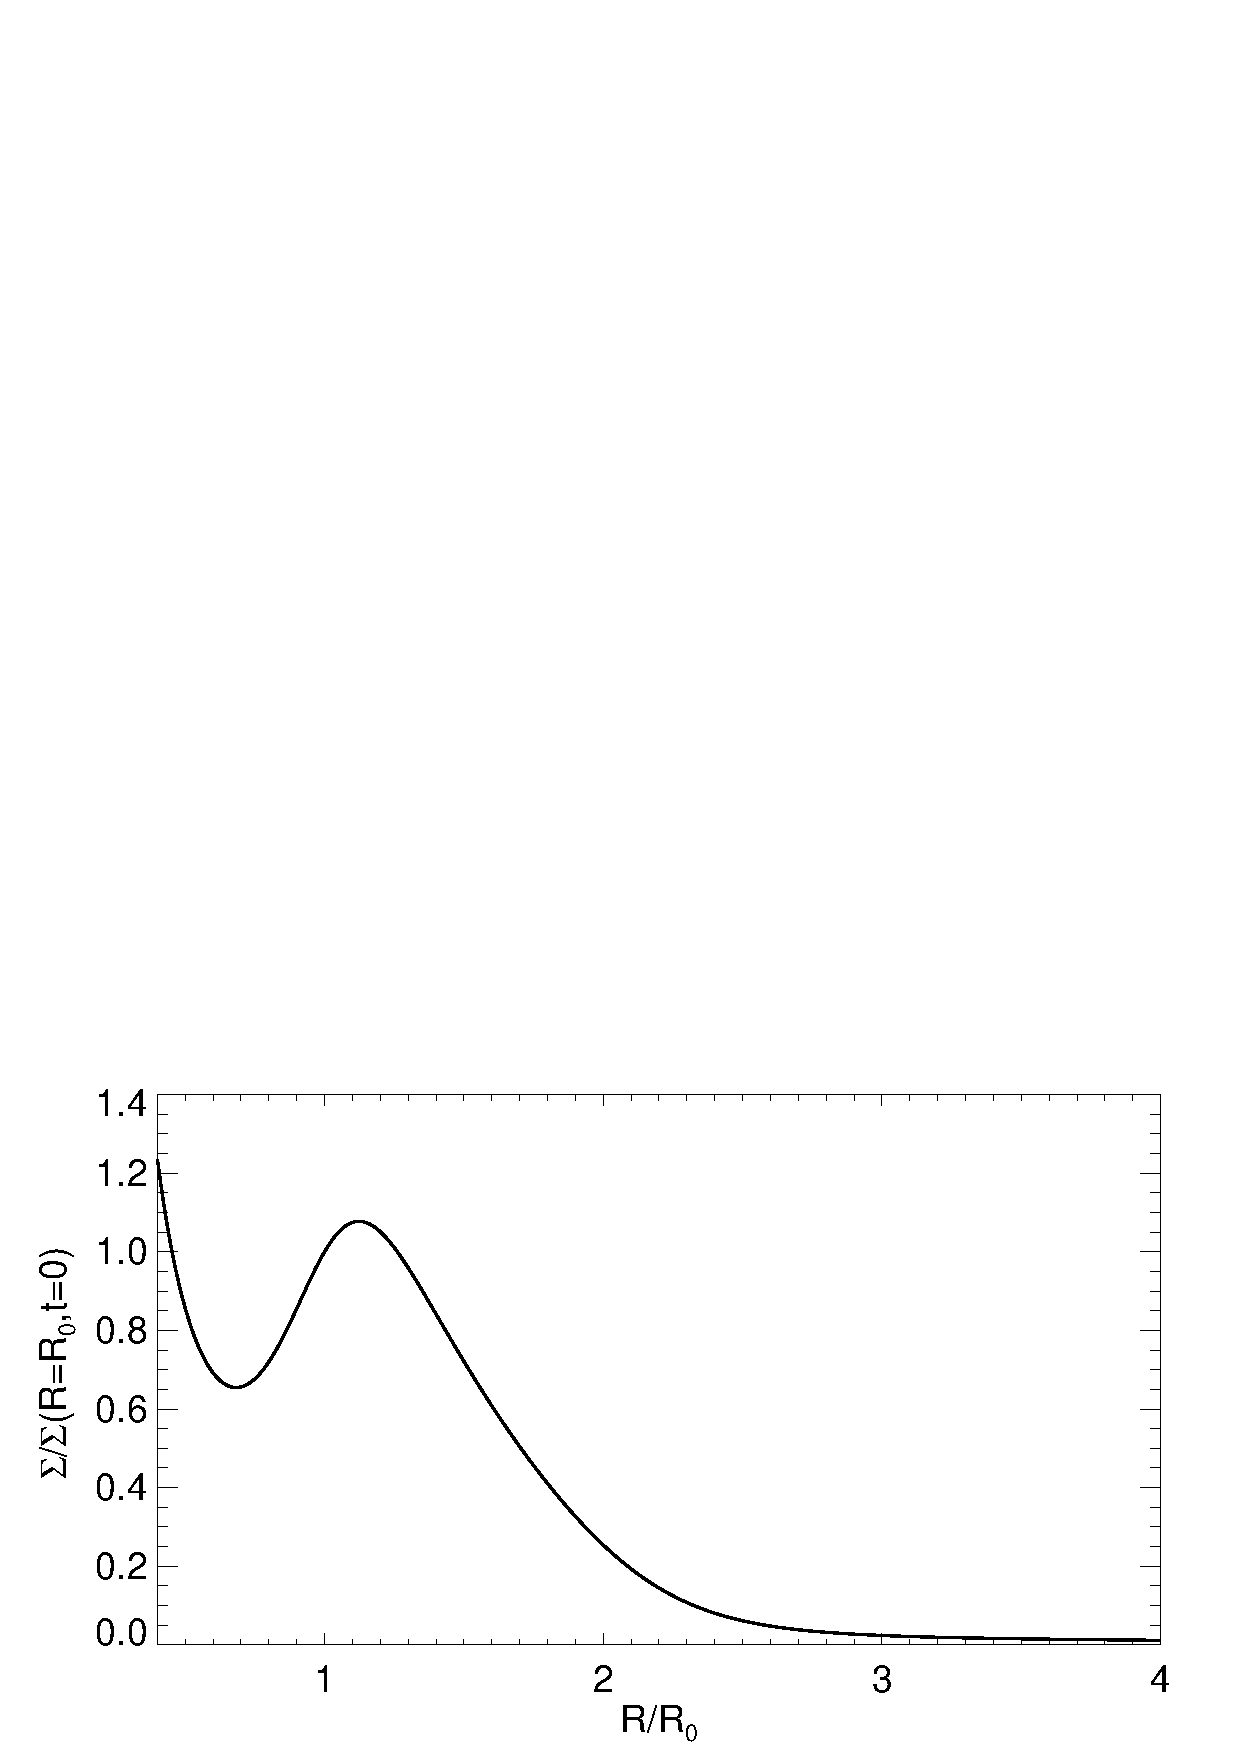
\includegraphics[width=\linewidth,clip=true,trim=0cm 1.7cm 0cm
  0cm]{figures/compare_profiles_dens000} 
  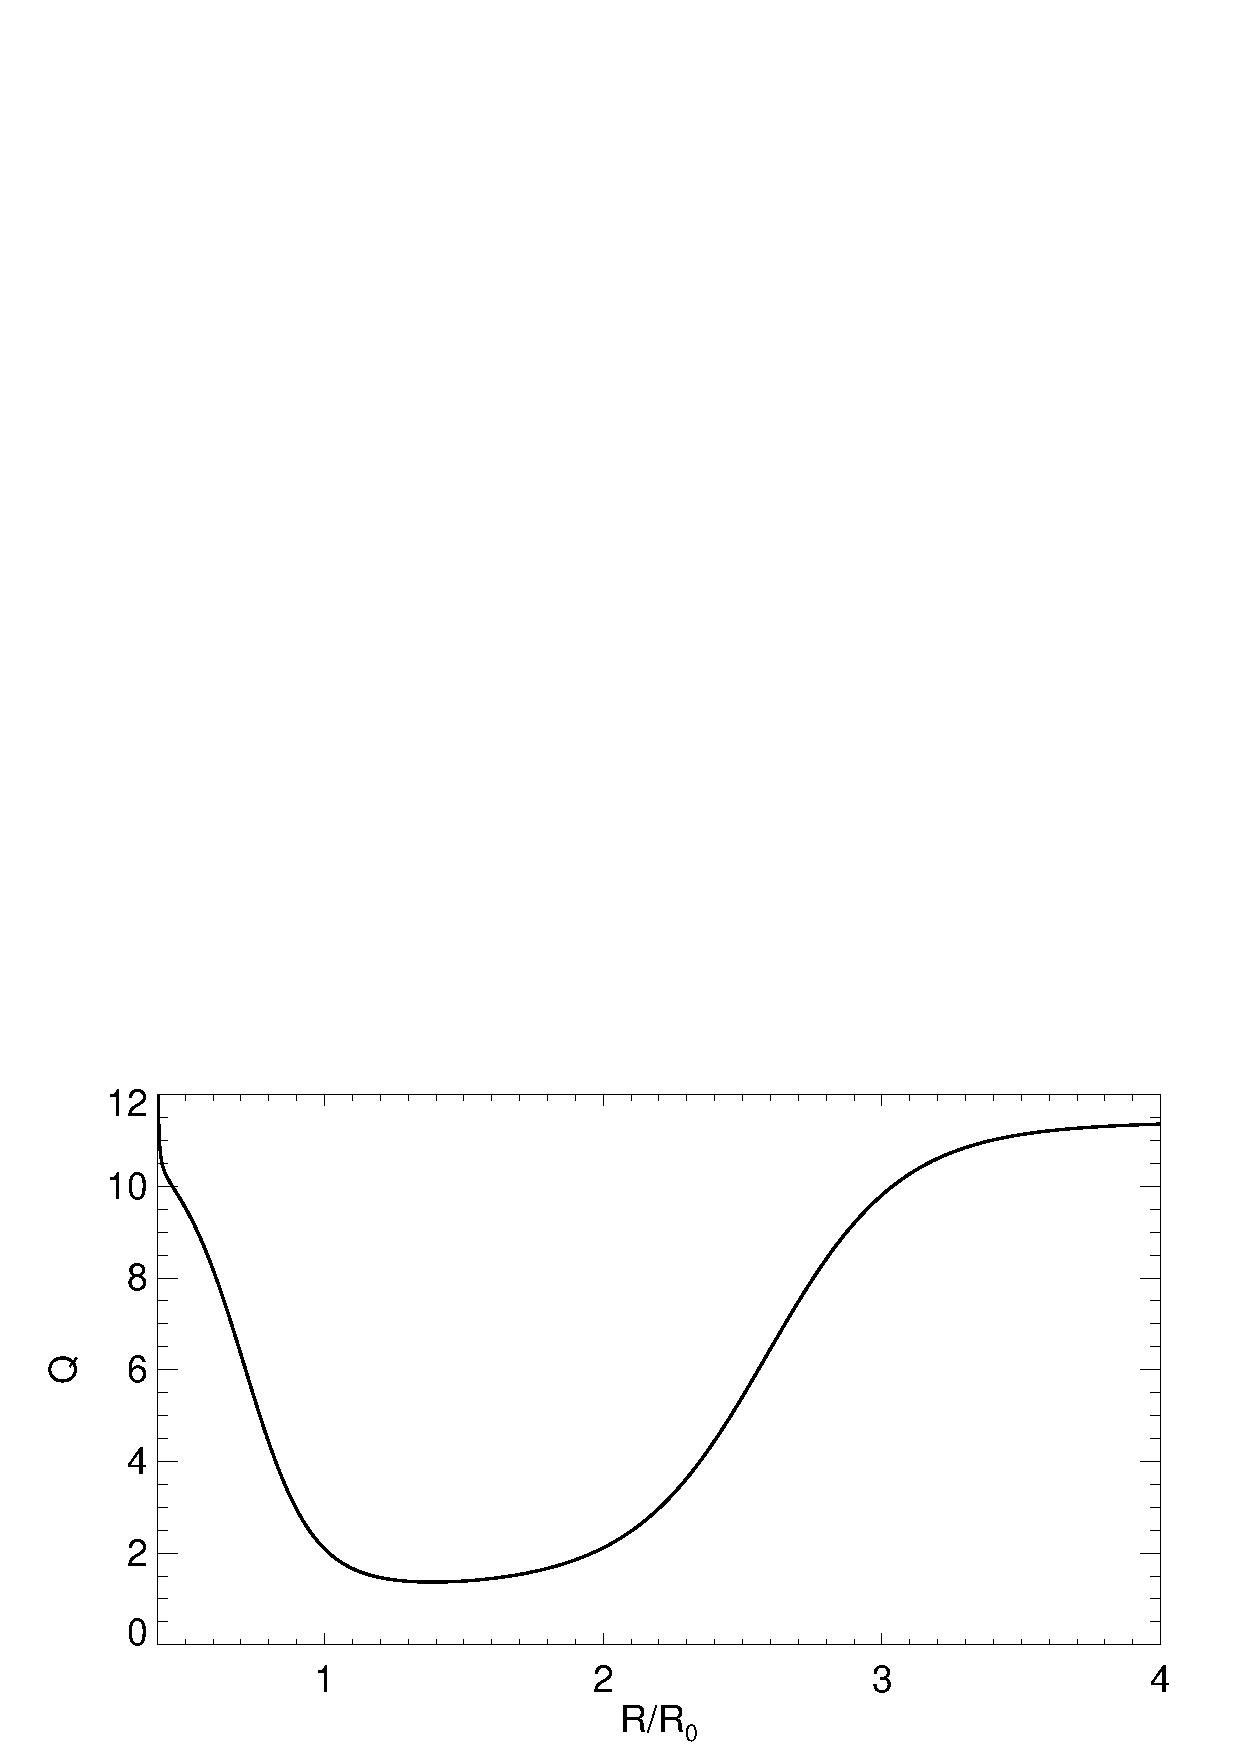
\includegraphics[width=\linewidth]{figures/compare_profiles_Q000}
  \caption{Fiducial profiles of the surface density (top) and Toomre
    parameter (bottom) used in this work.\label{initial_surf}}
\end{figure}


\section{Numerical methods}
%We will mostly employ 2D simulations in favour of resolution, but have
%also run some cases in 3D. We describe here the numerical setup used
%in each code. 
%introduce notation, terminlogy for each code 

We adopt computational units such that $G=M_*=R_0=1$. Time is measured
in the Keplerian orbital period at the reference radius, $P_0\equiv 
2\pi/\Omega_k(R_0)$.  

\subsection{FARGO}
Our primary code is FARGO with self-gravity \citep{baruteau08}. This
is a popular, simple finite-difference code for 2D discs. `FARGO' refers
to its azimuthal transport algorithm, which circumvents time-step
contraint set by the inner disc boundary. 
The 2D Poisson equation is solved in integral form 
\begin{align}\label{2d_grav}
  \Phi_{d,z=0}(R,\phi) = - \int
  \frac{G\Sigma(R^\prime,\phi^\prime)R^\prime dR^\prime d\phi^\prime}{\sqrt{R^2+R^{\prime 2} -
      2RR^\prime\cos{(\phi - \phi^\prime)} + \epsilon_g^2}} 
\end{align}
using Fast Fouier Transform (FFT), where $\epsilon_g$ is a softening
length to prevent a numerical singularity and the integration is taken
over the disc. The FFT approach requires
$\epsilon_g\propto R$ \citep{baruteau08}.  

The 2D disc occupies
$R\in[R_\mathrm{min},R_\mathrm{max}],\,\phi\in[0,2\pi]$ and is
divided into $(N_R,N_\phi)$ grids, logarithimically spaced in radius and
uniform spaced in azimuth. At radial boundaries we set the
hydrodynamic variables to their initial values.         

%poisson kernal integration, softening 
%where used?
%BC
\subsection{ZEUS-MP}
ZEUS-MP  is a general-purpose finite difference
code \citep{hayes06}. We use the code in 3D spherical geometry, covering
$r\in[r_\mathrm{min},r_\mathrm{max}]$, $\theta\in[\theta_\mathrm{min},\pi/2]$,
$\phi\in[0,2\pi]$. The vertical domain is chosen to cover $n_H$
scale-heights, i.e. $\tan{(\pi/2 - \theta_\mathrm{min})}/h=n_H$. 
The grid is logarithmically spaced in radius and uniformly spaced in the angular
coordinates. We assume reflectional symmetry across the midplane, and
apply relfective boundary conditions at radial boundaries and the
upper disc boundary.  

ZEUS-MP solves the 3D Poisson equation using a conjugate gradient
method. To suppliment boundary conditions for the linear solver, we
expand the boundary potential using in spherical harmonics $Y_{lm}$ 
as described in \cite{boss80}. The expansion is truncated at
$\lmax,\mmax$. This code was used in \cite{lin12b} for
self-gravitating disc-planet simulations.  

%used in lin 2012 
\subsection{PLUTO} 
PLUTO is a general-purpose Godunov code \citep{mignone07}. The grid
setup is the same as that adopted in ZEUS-MP above. We configure the
code similarly to that used in \cite{lin14}: piecewise linear
reconstruction, a Roe solver and second order Runge-Kutta time
integration. We also enable the FARGO algorithm for azimuthal
transport. 

We solve the 3D Poisson equation throughout the domain using spherical
harmonic expansion \citep{boss80}, as used for the boundary potential
in ZEUS-MP. This version of PLUTO was used in \cite{lin14b} for
self-gravitating disc-planet simulations, producing similar results to
that of ZEUS-MP and FARGO. 

%used in conference proceeding 

\section{Diagnostics}
 
\subsection{Evolution of non-axisymmetirc modes}
The disc evolution is quantified using mode amplitudes and angular
momenta as follows. We list the 2D definitions with obvious 3D generalisations. 
A hydrodynamic variable $f$ (e.g. $\Sigma$) is written as 
\begin{align}
  f(R,\phi) &= \sum_{m=-\infty}^{\infty}f_m(R)\exp{\ii m \phi} \notag\\
  &= f_0 + 2 \real\left[\sum_{m=1}^\infty f_m \exp{(\ii
      m\phi)}\right], 
\end{align}
where the $f_m$ may be obtained from Fourier transform in $\phi$. 

The non-axisymmetric surface density can be visualised with
\begin{align}
  \Delta \Sigma = \frac{\Sigma - \Sigma_{0}}{\Sigma_{0}}, 
\end{align}
while an individual mode as
\begin{align}
  \Delta\Sigma_m = \frac{2}{\Sigma_{00}} \real\left[\Sigma_m \exp{(\ii
      m\phi)}\right]
	\end{align}
where $\Sigma_{00} = \Sigma_0(t=0)$.  

The global mode amplitude is 
\begin{align}
  A_m = \frac{|C_m|}{M_{d0}}
\end{align}
where $M_{d0}$ is the initial disc mass and 
\begin{align}
  C_m = 2\pi\int_{R_1}^{R_2} \Sigma_m RdR, 
\end{align}
with integration limits chosen later. 

The time evolution of the $m^\mathrm{th}$ mode can be characterized by
assuming 
$\Sigma_m\propto\exp{(\ii \sigma t)}$, where
$\sigma = \omega - \ii\gamma$ is the complex frequency, $\omega$ is
the real frequency and $\gamma$ is the growth rate.
We estimate the growth rate as
\begin{align}
  \gamma = \frac{d\ln{A_m}}{dt},
\end{align}
and we estimate the real frequency by calculating the pattern speed
$\Omega_p = \omega/m$,
\begin{align}
  \Omega_p = \frac{d\phi_\mathrm{max}}{dt},
\end{align}
where $\phi_\mathrm{max}$ is the azimuthal co-ordinate of
$\mathrm{max}(\Delta\Sigma_m)$. 
%\begin{align}
%  \mathrm{max}\left\{2 \real\left[ \Sigma_m \exp{(\ii m
%        \phi)}\right]\right\},  

%other methods possible too 

\subsection{Angular momentum decomposition}
The total disc angular momentum in $R\in[R_1,R_2]$ is
\begin{align}
  J &= \int_{R_1}^{R_2}\int_0^{2\pi} \Sigma Rv_\phi RdRd\phi \notag\\
  &= 2\pi\int_{R_1}^{R_2}R\Sigma_0 v_{\phi0} R dR \notag\\ 
  &\phantom{=}+
  \sum_{m=1}^\infty2\pi\int_{R_1}^{R_2} 2R\real\left[\Sigma_m v_{\phi
      m}^*\right] RdR, \notag\\
  &= \sum_{m=0}^\infty \int_{R_1}^{R_2}  j_m(R) dR = \sum_{m=0}^\infty J_m. 
\end{align}
where $^*$ denotes complex conjugation, and we idenfity $J_m$ as the angular momentum 
associated with the $m^\mathrm{th}$ mode, and $j_m$ the associated
angular momentum per unit length. 

\subsection{Linear density waves}\label{wkb}
We will also use linear density wave theory to interpret
simulation data. Here, we follow conventions in \cite{shu91} and quote
results therein. The dispersion relation for tightly-wound density
waves of the form 
$\exp{[\ii(\omega t - m \phi + kR)]}$ in a razor-thin
isothermal disc is 
\begin{align}\label{dispersion}
  (\omega - m\Omega)^2 = \kappa^2 + k^2c_s^2 - 2\pi G \Sigma |k|, 
\end{align}
where $\kappa^2 = R^{-3}\p_R(R^4\Omega^2)$ is the square of the epicycle frequency, 
and $k$ is a real wavenumber such that $|kR|\gg1$. 

Given the pattern speed $\Omega_p$,
Eq. \ref{dispersion} can be solved for $|k|$, 
\begin{align}\label{wavenumber}
  \frac{|k|}{k_T} = \frac{2}{Q^2}\left[1 \pm \sqrt{1 -
      Q^2(1-\nu^2)}\right], 
\end{align}
where 
\begin{align}
  k_T \equiv \frac{\kappa^2}{2\pi G \Sigma}
\end{align}
is a characteristic wavenumber, 
\begin{align}
  Q \equiv \frac{c_s\kappa}{\pi G \Sigma}
\end{align}
is the usual Toomre parameter, and
\begin{align}
  \nu \equiv \frac{(\omega - m\Omega)}{\kappa}
\end{align}
is a dimensionless frequency.  The upper (lower) signs in
Eq. \ref{wavenumber} correspond to short (long) waves.  

The \emph{co-rotation radius} $R_c$ is where the pattern speed matches
the fluid rotation,
\begin{align}
  \Omega(R_c) = \Omega_p.
\end{align}
\emph{Lindblad resonances} $R_L$ occurs where
\begin{align}
  \nu^2(R_L) = 1. 
\end{align}
Finally, \emph{Q-barriers} occur at radii $R_{Qb}$ where
\begin{align}
  Q^2(R_{Qb})\left[1-\nu^2(R_{Qb})\right] = 1.  
\end{align}
According to Eq. \ref{wavenumber}, purely wave-like solutions with
real $k$ are only possible when $Q^2(1-\nu^2)\leq1$.  

% We use Eq. \ref{wavenumber} to set trailing long waves as
% perturbations, i.e. $k/k_T = -2Q^{-2}\left[1 - \sqrt{1 -
%     Q^2(1-\nu^2)}\right]$.  
% We only apply the perturbations where $Q^{-2}(1-\nu^2)<1$. 

% The amplitude of the surface density and velocity perturbations are
% related by
% \begin{align}
%   &\left(\omega - m\Omega\right)\delta\Sigma + k\Sigma\delta v_R= 0,\\
%   &\frac{\kappa^2}{2\Omega} \delta v_R + \ii (\omega - m\Omega)\delta
%   v_\phi=0. 
% \end{align}
% We set $\delta\Sigma = 10^{-3}\Sigma$ and $(\delta v_R, \delta
% v_\phi)$ accordingly.   

% %Having chosen the wave frequency and set the wavenumber according to
% %the above, 


